\section{寄存器描述}
\regover{
{\hyperref[HBN-HBN-CTL]{HBN\_CTL}}&
\\
\hline
{\hyperref[HBN-HBN-TIME-L]{HBN\_TIME\_L}}&
\\
\hline
{\hyperref[HBN-HBN-TIME-H]{HBN\_TIME\_H}}&
\\
\hline
{\hyperref[HBN-RTC-TIME-L]{RTC\_TIME\_L}}&
\\
\hline
{\hyperref[HBN-RTC-TIME-H]{RTC\_TIME\_H}}&
\\
\hline
{\hyperref[HBN-HBN-IRQ-MODE]{HBN\_IRQ\_MODE}}&
\\
\hline
{\hyperref[HBN-HBN-IRQ-STAT]{HBN\_IRQ\_STAT}}&
\\
\hline
{\hyperref[HBN-HBN-IRQ-CLR]{HBN\_IRQ\_CLR}}&
\\
\hline
{\hyperref[HBN-HBN-PIR-CFG]{HBN\_PIR\_CFG}}&
\\
\hline
{\hyperref[HBN-HBN-PIR-VTH]{HBN\_PIR\_VTH}}&
\\
\hline
{\hyperref[HBN-HBN-PIR-INTERVAL]{HBN\_PIR\_INTERVAL}}&
\\
\hline
{\hyperref[HBN-HBN-BOR-CFG]{HBN\_BOR\_CFG}}&
\\
\hline
{\hyperref[HBN-HBN-GLB]{HBN\_GLB}}&
\\
\hline
{\hyperref[HBN-HBN-SRAM]{HBN\_SRAM}}&
\\
\hline
{\hyperref[HBN-HBN-PAD-CTRL-0]{HBN\_PAD\_CTRL\_0}}&
\\
\hline
{\hyperref[HBN-HBN-PAD-CTRL-1]{HBN\_PAD\_CTRL\_1}}&
\\
\hline
{\hyperref[HBN-vbat-ldo]{vbat\_ldo}}&
\\
\hline
{\hyperref[HBN-rc32k-ctrl0]{rc32k\_ctrl0}}&
\\
\hline
{\hyperref[HBN-xtal32k]{xtal32k}}&
\\
\hline
}

\subsection{HBN\_CTL}
\label{HBN-HBN-CTL}
地址:0x2000f000
 \begin{figure}[H]
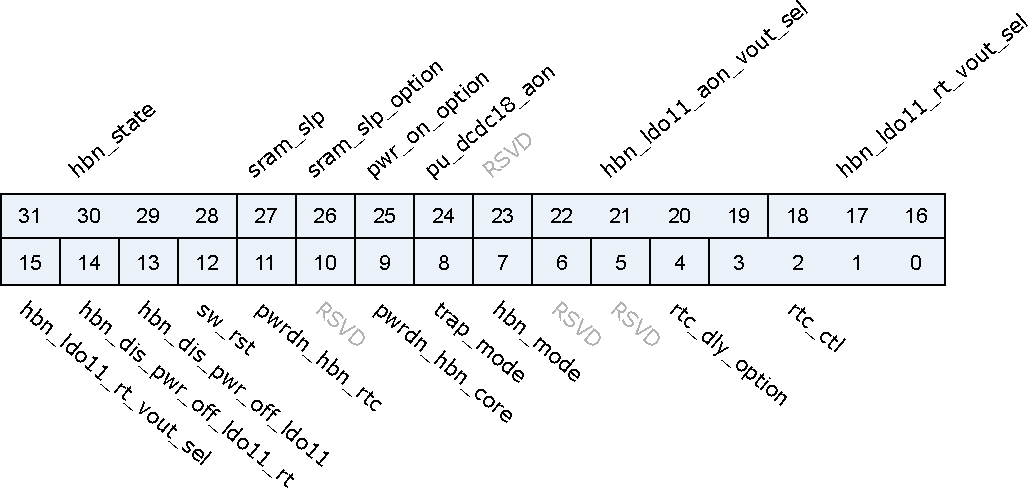
\includegraphics{HBN_HBN_CTL.pdf}
\end{figure}

\regdes{31:28&hbn\_state&r&4'h0&SW polling until 0 (default 4'h3 @pwron)\\\hline
27&sram\_slp&r&1'b0&SW polling until 0 (default 1'b1 @pwron)\\\hline
26&sram\_slp\_option&r/w&0&\\\hline
25&pwr\_on\_option&r/w&0&\\\hline
24&pu\_dcdc18\_aon&r/w&1&Power On DCDC18 during Power On Sequence (require 400~800us)\\\hline
23&RSVD& & & \\\hline
22:19&hbn\_ldo11\_aon\_vout\_sel&r/w&4'hA&VDD11\_AON Voltage Out Select @ Enter hibernate\\\hline
18:15&hbn\_ldo11\_rt\_vout\_sel&r/w&4'hA&VDD11\_RT   Voltage Out Select @ Enter hibernate\\\hline
14&hbn\_dis\_pwr\_off\_ldo11\_rt&r/w&0&Set 1 to disable power off VDDCORE\_RT at HBN mode (for low power)\\\hline
13&hbn\_dis\_pwr\_off\_ldo11&r/w&0&Set 1 to disable power off VDDCORE at HBN mode (for debug)\\\hline
12&sw\_rst&r/w&0&soft reset\\\hline
11&pwrdn\_hbn\_rtc&r/w&0&Power Off HBN RTC @ Enter hibernate\\\hline
10&RSVD& & & \\\hline
9&pwrdn\_hbn\_core&r/w&0&Power Off HBN Core @ Enter hibernate\\\hline
8&trap\_mode&r&0&Boot Strap  0: Flash,  1: UART or SDIO\\\hline
7&hbn\_mode&w&0&Enter hibernate\\\hline
6:5&RSVD& & & \\\hline
4&rtc\_dly\_option&r/w&0&\\\hline
3:0&rtc\_ctl&r/w&4'h0&[6:4] Slow LED, x/0.25/0.5/1/2/4/8/16 seconds (move to 0x38) \par [3] rtc long time 0~353days (bit 39~13 compare) \par [2] rtc short time 0~488s (bit 23~0 compare) \par [1] rtc time 0~353days (bit 39~0 compare) \par [0] rtc enable
\\\hline

}
\subsection{HBN\_TIME\_L}
\label{HBN-HBN-TIME-L}
地址:0x2000f004
 \begin{figure}[H]
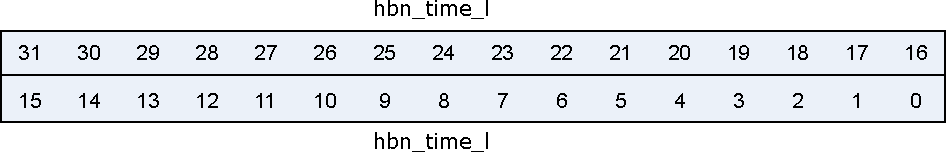
\includegraphics{HBN_HBN_TIME_L.pdf}
\end{figure}

\regdes{31:0&hbn\_time\_l&r/w&32'h0&RTC timer compare bit 31:0\\\hline

}
\subsection{HBN\_TIME\_H}
\label{HBN-HBN-TIME-H}
地址:0x2000f008
 \begin{figure}[H]
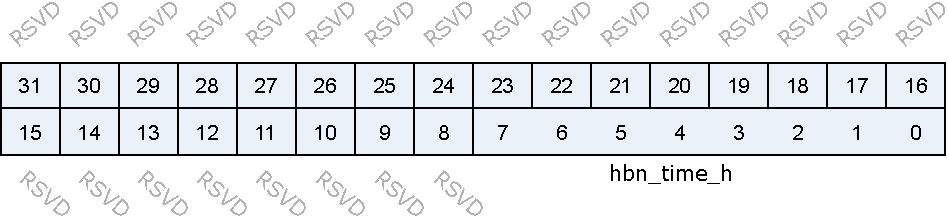
\includegraphics{HBN_HBN_TIME_H.pdf}
\end{figure}

\regdes{31:8&RSVD& & & \\\hline
7:0&hbn\_time\_h&r/w&8'h0&RTC timer compare bit 39:32\\\hline

}
\subsection{RTC\_TIME\_L}
\label{HBN-RTC-TIME-L}
地址:0x2000f00c
 \begin{figure}[H]
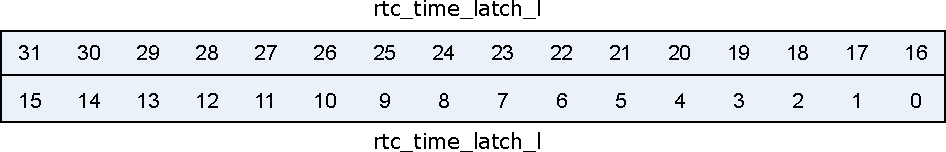
\includegraphics{HBN_RTC_TIME_L.pdf}
\end{figure}

\regdes{31:0&rtc\_time\_latch\_l&r&32'h0&RTC time latched value bit 31:0\\\hline

}
\subsection{RTC\_TIME\_H}
\label{HBN-RTC-TIME-H}
地址:0x2000f010
 \begin{figure}[H]
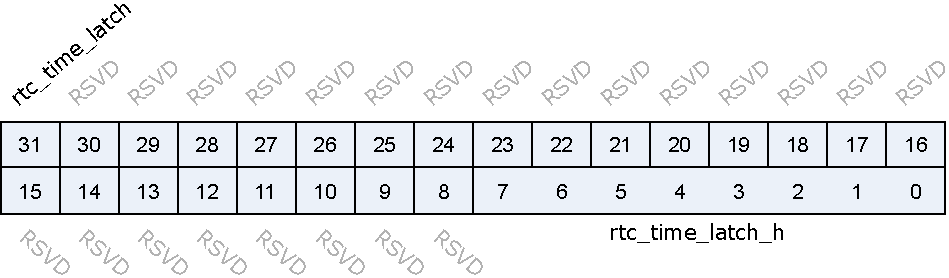
\includegraphics{HBN_RTC_TIME_H.pdf}
\end{figure}

\regdes{31&rtc\_time\_latch&w&0&RTC time latch for SW read\\\hline
30:8&RSVD& & & \\\hline
7:0&rtc\_time\_latch\_h&r&8'h0&RTC time latched value bit 39:32\\\hline

}
\subsection{HBN\_IRQ\_MODE}
\label{HBN-HBN-IRQ-MODE}
地址:0x2000f014
 \begin{figure}[H]
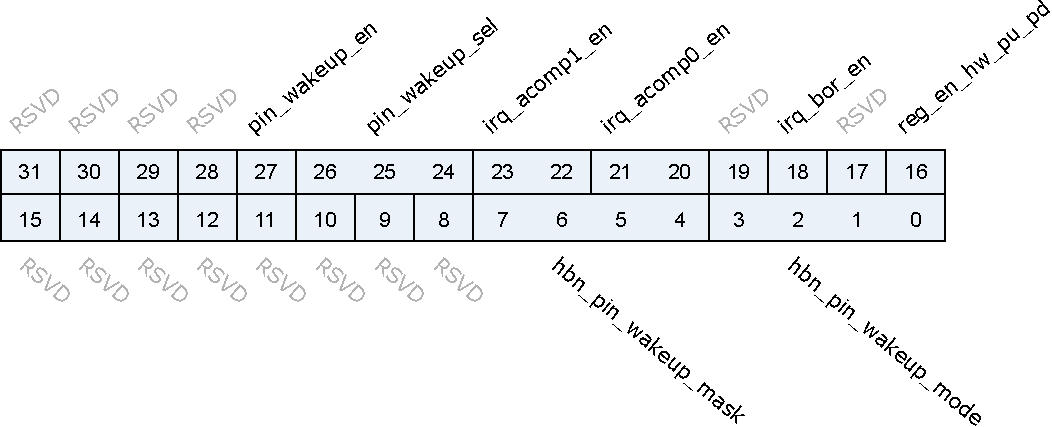
\includegraphics{HBN_HBN_IRQ_MODE.pdf}
\end{figure}

\regdes{31:28&RSVD& & & \\\hline
27&pin\_wakeup\_en&r/w&0&Pin wakeup delay enable\\\hline
26:24&pin\_wakeup\_sel&r/w&3'd3&Pin wakeup delay 1~7 sec\\\hline
23:22&irq\_acomp1\_en&r/w&0&enable acomp1 interrupt [20] posedge [21] negedge\\\hline
21:20&irq\_acomp0\_en&r/w&0&enable acomp0 interrupt [20] posedge [21] negedge\\\hline
19&RSVD& & & \\\hline
18&irq\_bor\_en&r/w&0&enable brown-out interrupt\\\hline
17&RSVD& & & \\\hline
16&reg\_en\_hw\_pu\_pd&r/w&1&1:  Pull GPIO17 @ pwr\_on and pwr\_rst 0 : no pull\\\hline
15:8&RSVD& & & \\\hline
7:4&hbn\_pin\_wakeup\_mask&r/w&4'b0&mask hbn\_pin\_wakeup\_event\\\hline
3:0&hbn\_pin\_wakeup\_mode&r/w&4'b0101&hbn\_pin\_wakeup mode  \par 0000 : sync falling edge trigger \par 0001 : sync rising edge trigger \par 0010 : sync low level trigger \par 0011 : sync high level trigger \par 01xx : sync rising \& falling edge trigger \par 1000 : async falling edge trigger \par 1001 : async rising edge trigger \par 1010 : async low level trigger \par 1011 : async high level trigger
\\\hline

}
\subsection{HBN\_IRQ\_STAT}
\label{HBN-HBN-IRQ-STAT}
地址:0x2000f018
 \begin{figure}[H]
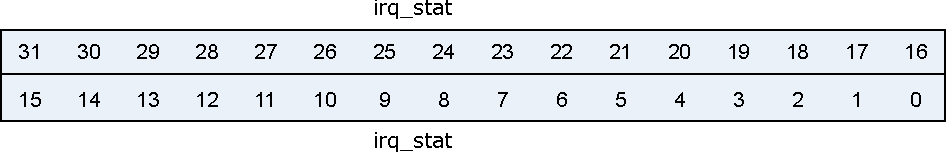
\includegraphics{HBN_HBN_IRQ_STAT.pdf}
\end{figure}

\regdes{31:0&irq\_stat&r&0&[22] acomp1 \par [20] acomp0 \par [18] brown-out \par [17] irq\_pir state \par [16] irq\_rtc state \par [3:0] hbn\_pin\_wakeup state (GPIO19/18/17/16)
\\\hline

}
\subsection{HBN\_IRQ\_CLR}
\label{HBN-HBN-IRQ-CLR}
地址:0x2000f01c
 \begin{figure}[H]
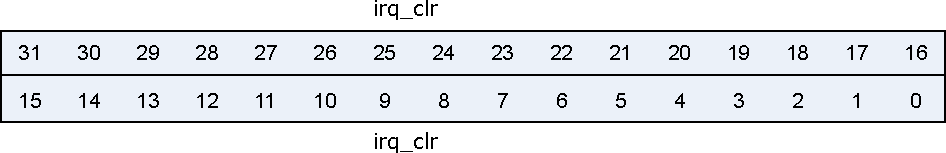
\includegraphics{HBN_HBN_IRQ_CLR.pdf}
\end{figure}

\regdes{31:0&irq\_clr&w&0&[22] irq\_acomp1 clear \par [20] irq\_acomp0 clear \par [18] irq\_bor clear \par [17] irq\_pir clear \par [16] irq\_rtc clear \par [3:0] hbn\_pin\_wakeup state (GPIO19/18/17/16)
\\\hline

}
\subsection{HBN\_PIR\_CFG}
\label{HBN-HBN-PIR-CFG}
地址:0x2000f020
 \begin{figure}[H]
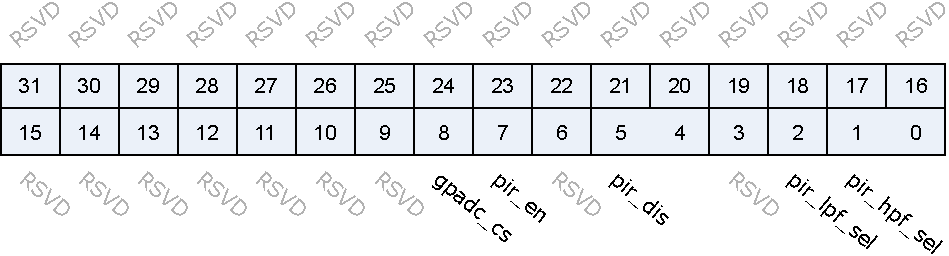
\includegraphics{HBN_HBN_PIR_CFG.pdf}
\end{figure}

\regdes{31:9&RSVD& & & \\\hline
8&gpadc\_cs&r/w&0&GPADC clock source select signal \par 0: 32MHz clock \par 1: PIR clock (f32k\_clk)
\\\hline
7&pir\_en&r/w&0&pir enable\\\hline
6&RSVD& & & \\\hline
5:4&pir\_dis&r/w&0&pir disable \par [4] low -> high won't trigger interrupt \par [5] high -> low won't trigger interrupt
\\\hline
3&RSVD& & & \\\hline
2&pir\_lpf\_sel&r/w&0&0: /1.  1:/2\\\hline
1:0&pir\_hpf\_sel&r/w&0&0: 1-z\^-1,  1: 1-z\^-2,  0: 2-z\^-3\\\hline

}
\subsection{HBN\_PIR\_VTH}
\label{HBN-HBN-PIR-VTH}
地址:0x2000f024
 \begin{figure}[H]
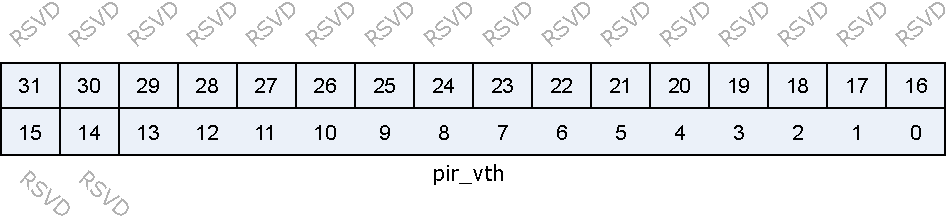
\includegraphics{HBN_HBN_PIR_VTH.pdf}
\end{figure}

\regdes{31:14&RSVD& & & \\\hline
13:0&pir\_vth&r/w&14'h3ff&PIR compare threshold\\\hline

}
\subsection{HBN\_PIR\_INTERVAL}
\label{HBN-HBN-PIR-INTERVAL}
地址:0x2000f028
 \begin{figure}[H]
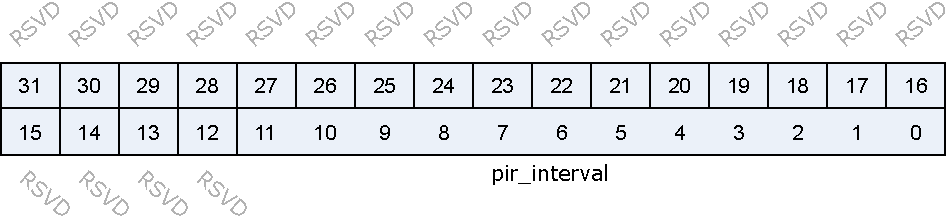
\includegraphics{HBN_HBN_PIR_INTERVAL.pdf}
\end{figure}

\regdes{31:12&RSVD& & & \\\hline
11:0&pir\_interval&r/w&12'd2621&pir\_lpf\_sel = 0: 32768 / (pir\_interval+1) Hz,  default 12.5Hz (~80ms) \par pir\_lpf\_sel = 1: 32768 / (pir\_interval*2+1) Hz,  default 6.25Hz (~160ms)
\\\hline

}
\subsection{HBN\_BOR\_CFG}
\label{HBN-HBN-BOR-CFG}
地址:0x2000f02c
 \begin{figure}[H]
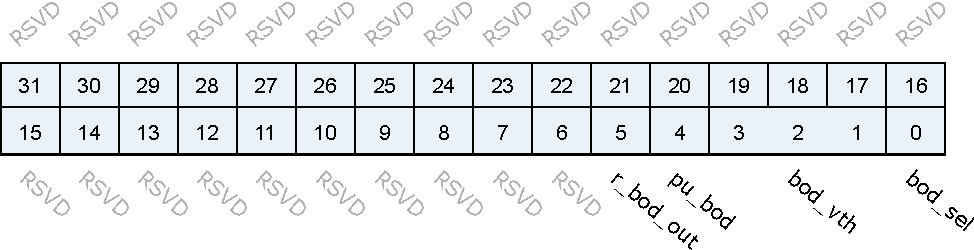
\includegraphics{HBN_HBN_BOR_CFG.pdf}
\end{figure}

\regdes{31:6&RSVD& & & \\\hline
5&r\_bod\_out&r&1'h0&\\\hline
4&pu\_bod&r/w&1'h0&Power up Brown Out Reset\\\hline
3:1&bod\_vth&r/w&3'h5&bod threshold \par 000: 2.05V, \par 001: 2.10V, \par 010: 2.15V, \par 011: 2.20V, \par 100: 2.25V, \par 101: 2.30V, \par 110: 2.35V, \par 111: 2.40V
\\\hline
0&bod\_sel&r/w&1'h0&0: POR is independent of BOD,  1: POR is relevant to BOD\\\hline

}
\subsection{HBN\_GLB}
\label{HBN-HBN-GLB}
地址:0x2000f030
 \begin{figure}[H]
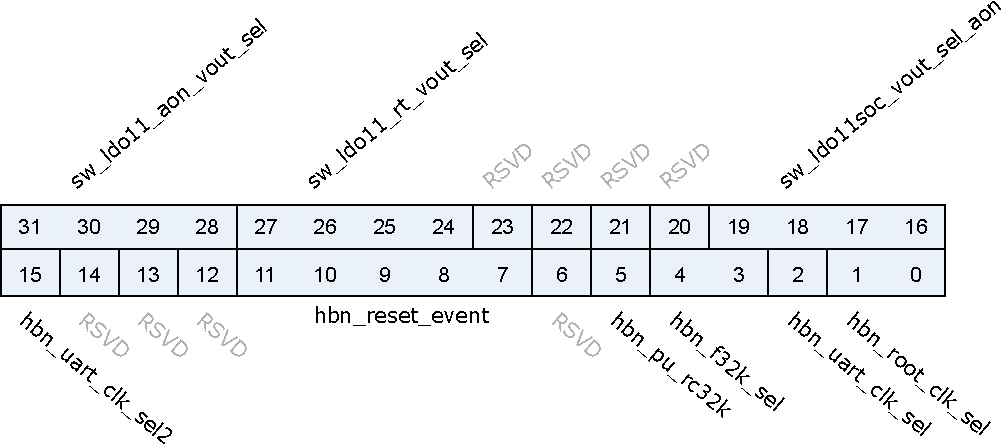
\includegraphics{HBN_HBN_GLB.pdf}
\end{figure}

\regdes{31:28&sw\_ldo11\_aon\_vout\_sel&r/w&4'ha&aon ldo output voltage external control: \par 0:0.70V, 1:0.70V, 2:0.70V, 3:0.75V, 4:0.80V, 5:0.85V, 6:0.9V, 7:0.95V \par 8:1.0V, 9:1.05V, 10:1.1V, 11:1.15V, 12:1.2V, 13:1.25V, 14:1.3V, 15:1.35V
\\\hline
27:24&sw\_ldo11\_rt\_vout\_sel&r/w&4'ha&ldo output voltage external control: \par 0:0.70V, 1:0.70V, 2:0.70V, 3:0.75V, 4:0.80V, 5:0.85V, 6:0.9V, 7:0.95V \par 8:1.0V, 9:1.05V, 10:1.1V, 11:1.15V, 12:1.2V, 13:1.25V, 14:1.3V, 15:1.35V
\\\hline
23:20&RSVD& & & \\\hline
19:16&sw\_ldo11soc\_vout\_sel\_aon&r/w&4'hA&vdd11soc output voltage selection\\\hline
15&hbn\_uart\_clk\_sel2&r/w&0&UART clock selection2 from HBN  \par (0 : result of hbn\_uart\_clk\_sel (bclk or MUX 160MHz),  \par  1: XCLK (XTAL or RC32M))
\\\hline
14:12&RSVD& & & \\\hline
11:7&hbn\_reset\_event&r&5'b0&[4] : bor\_out\_ event \par [3] : pwr\_rst\_n event \par [2] : sw\_rst event \par [1] : por\_out event \par [0] : watch dog reset
\\\hline
6&RSVD& & & \\\hline
5&hbn\_pu\_rc32k&r/w&1&0: Turn off rc32k during rtc power domain off, 1: Don't turn off rc32k (move to RTC Domain)\\\hline
4:3&hbn\_f32k\_sel&r/w&0&32KHz clock source selection (0: RC32K  1: XTAL 32K  3: DIG 32K)\\\hline
2&hbn\_uart\_clk\_sel&r/w&0&UART clock selection from HBN (0:bclk  1:muxpll\_160m\_clk)\\\hline
1:0&hbn\_root\_clk\_sel&r/w&0&root clock source selection (0: RC32M  1: XTAL  2/3: PLL)\\\hline

}
\subsection{HBN\_SRAM}
\label{HBN-HBN-SRAM}
地址:0x2000f034
 \begin{figure}[H]
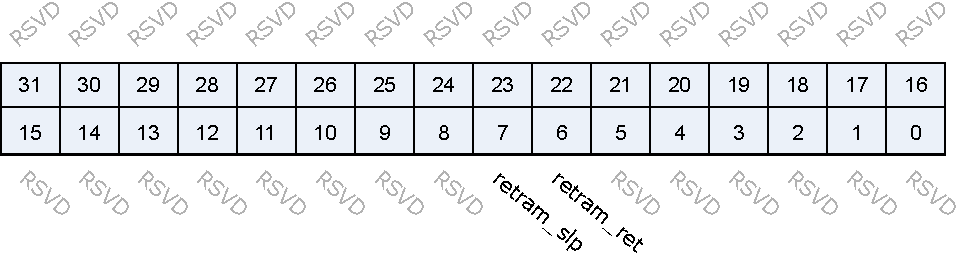
\includegraphics{HBN_HBN_SRAM.pdf}
\end{figure}

\regdes{31:8&RSVD& & & \\\hline
7&retram\_slp&r/w&0&\\\hline
6&retram\_ret&r/w&0&\\\hline
5:0&RSVD& & & \\\hline

}
\subsection{HBN\_PAD\_CTRL\_0}
\label{HBN-HBN-PAD-CTRL-0}
地址:0x2000f038
 \begin{figure}[H]
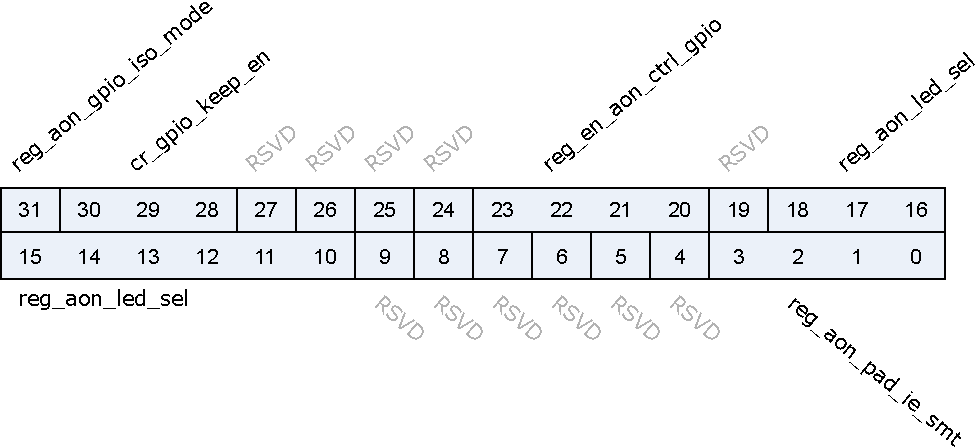
\includegraphics{HBN_HBN_PAD_CTRL_0.pdf}
\end{figure}

\regdes{31&reg\_aon\_gpio\_iso\_mode&r/w&0&1: HW Keep GPIO  @ PDS or HBN Mode \par 0 : No Keep GPIO @ PDS or HBN Mode 
\\\hline
30:28&cr\_gpio\_keep\_en&r/w&0&if cr\_aon\_ctrl\_gpio\_latch=1, can use bit to enable or disable IO latch function at enter HBN Mode \par [0] : GPIO0~15 \par [1] : GPIO20~36 \par [2] : GPIO16~19
\\\hline
27:24&RSVD& & & \\\hline
23:20&reg\_en\_aon\_ctrl\_gpio&&4'h0&AON GPIO16~19 Control by AON HW :  \par [23] :GPIO19  \par [22]: GPIO18  \par [21]: GPIO17(can be muxed to be XTAL32K) \par [20]: GPIO16(can be muxed to be  XTAL32K)
\\\hline
19&RSVD& & & \\\hline
18:10&reg\_aon\_led\_sel&&9'h000&(if corresponding  AON GPIO controlled by AON HW)  \par Always on PAD Output Slow LED, x/0.25/0.5/1/2/4/8/16 seconds \par [12:10] (for GPIO16)       : reg\_aon\_led1\_sel \par [15:13] (for GPIO17)       : reg\_aon\_led2\_sel \par [18:16] (for GPIO18/19) : reg\_aon\_led3\_sel \par 1 : 0.25sec \par 2 : 0.5sec \par 3: 1 sec \par 4:  2sec \par 5: 4 sec \par 6 : 8sec \par 7 :16sec
\\\hline
9:4&RSVD& & & \\\hline
3:0&reg\_aon\_pad\_ie\_smt&&4'h0&Always on PAD IE/SMT (if corresponding  AON GPIO controlled by AON HW)  \par [3] : GPIO19 \par [2] : GPIO18 \par [1] : GPIO17 \par [0] : GPIO16
\\\hline

}
\subsection{HBN\_PAD\_CTRL\_1}
\label{HBN-HBN-PAD-CTRL-1}
地址:0x2000f03c
 \begin{figure}[H]
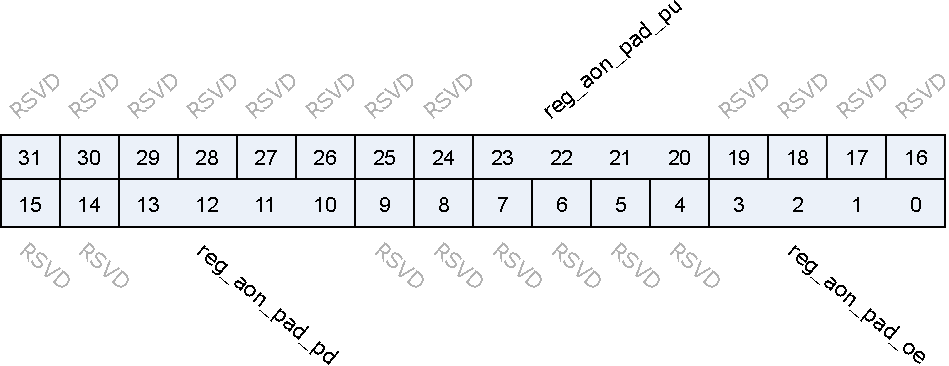
\includegraphics{HBN_HBN_PAD_CTRL_1.pdf}
\end{figure}

\regdes{31:24&RSVD& & & \\\hline
23:20&reg\_aon\_pad\_pu&&4'h0&Always on PAD PU (if corresponding  AON GPIO controlled by AON HW)  \par [23] : GPIO19 \par [22] : GPIO18 \par [21] : GPIO17 \par [20] : GPIO16
\\\hline
19:14&RSVD& & & \\\hline
13:10&reg\_aon\_pad\_pd&&4'h0&Always on PAD PD (if corresponding  AON GPIO controlled by AON HW)  \par [13] : GPIO19 \par [12] : GPIO18 \par [11] : GPIO17 \par [10] : GPIO16
\\\hline
9:4&RSVD& & & \\\hline
3:0&reg\_aon\_pad\_oe&&4'h0&Always on PAD OE (if corresponding  AON GPIO controlled by AON HW)  \par [3] : GPIO19 \par [2] : GPIO18 \par [1] : GPIO17 \par [0] : GPIO16
\\\hline

}
\subsection{vbat\_ldo}
\label{HBN-vbat-ldo}
地址:0x2000f040
 \begin{figure}[H]
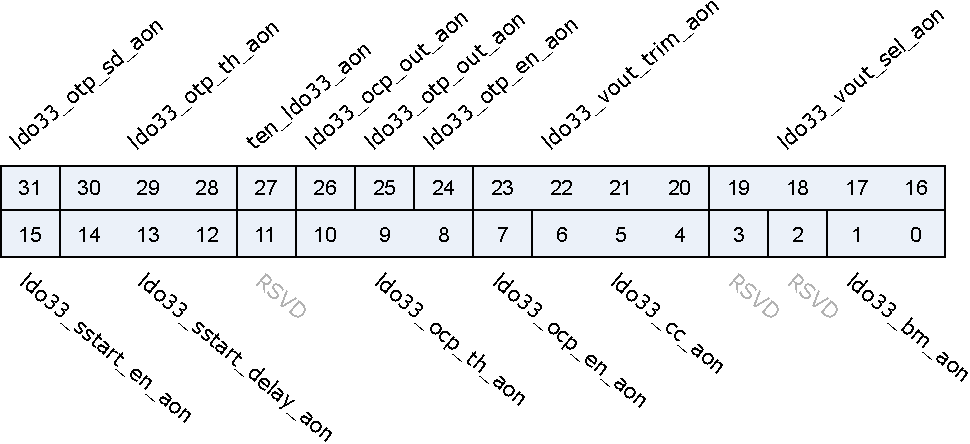
\includegraphics{HBN_vbat_ldo.pdf}
\end{figure}

\regdes{31&ldo33\_otp\_sd\_aon&r/w&1'h0&0: donot pulldown ldo33 when OTP happens, 1: pulldown ldo33 when OTP happens\\\hline
30:28&ldo33\_otp\_th\_aon&r/w&3'h7&OTP temperature threshold selection: \par 0: 125C, \par 1: 150C, \par 2: 175C, \par 3: 200C, \par 4: 200C, \par . \par 7: 200C
\\\hline
27&ten\_ldo33\_aon&r/w&1'h0&\\\hline
26&ldo33\_ocp\_out\_aon&r&1'h0&OCP signal\\\hline
25&ldo33\_otp\_out\_aon&r&1'h0&OTP signal\\\hline
24&ldo33\_otp\_en\_aon&r/w&1'h1&enable Over Temperature Protection circuit in vbat\_top\\\hline
23:20&ldo33\_vout\_trim\_aon&r/w&4'h8&output voltage trim: 1% per step \par 0: 91%, \par . \par 7: 99%, \par 8: 100%, \par 9: 101%, \par . \par f: 108%
\\\hline
19:16&ldo33\_vout\_sel\_aon&r/w&4'hb&avdd33\_out voltage selection: \par 0: 2.10, \par 1: 2.20, \par 2: 2.30, \par 3: 2.40, \par 4: 2.50, \par 5: 2.70, \par 6: 2.90, \par 7: 3.00, \par 8: 3.10, \par 9: 3.20, \par a: 3.25, \par b: 3.30, \par c: 3.35, \par d: 3.40, \par e: 3.50, \par f: 3.60
\\\hline
15&ldo33\_sstart\_en\_aon&r/w&1'h1&enable Soft-start circuit in vbat\_top\\\hline
14:12&ldo33\_sstart\_delay\_aon&r/w&3'h3&Sstart time selection: \par 0: 200us,  \par 1: 290us, \par 2: 390us, \par 3: 480us, \par 4: 580us, \par 5: 670us, \par 6: 770us, \par 7: 860us
\\\hline
11&RSVD& & & \\\hline
10:8&ldo33\_ocp\_th\_aon&r/w&3'h5&OCP current threshold selection: \par 0: 0.5A,  \par 1: 0.6A, \par 2: 0.8A, \par 3: 1.0A, \par 4: 1.2A, \par 5: 1.5A, \par 6: 2.0A, \par 7: 2.0A
\\\hline
7&ldo33\_ocp\_en\_aon&r/w&1'h1&enable Over Current Protection circuit in vbat\_top\\\hline
6:4&ldo33\_cc\_aon&r/w&3'h1&Compensation Capacitance selection\\\hline
3:2&RSVD& & & \\\hline
1:0&ldo33\_bm\_aon&r/w&2'h1&Bias mode selection\\\hline

}
\subsection{rc32k\_ctrl0}
\label{HBN-rc32k-ctrl0}
地址:0x2000f200
 \begin{figure}[H]
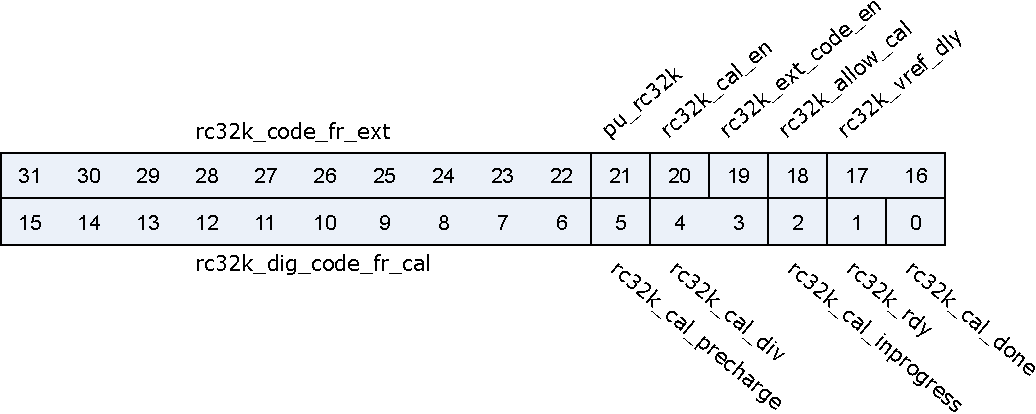
\includegraphics{HBN_rc32k_ctrl0.pdf}
\end{figure}

\regdes{31:22&rc32k\_code\_fr\_ext&r/w&10'h12C&External code In for frequency setting\\\hline
21&pu\_rc32k&r/w&1&Power up 32k oscillator (Useless in 616)\\\hline
20&rc32k\_cal\_en&r/w&0&Enable calibration of 32k oscillator\\\hline
19&rc32k\_ext\_code\_en&r/w&1&Allow external code in to go into the ckt\\\hline
18&rc32k\_allow\_cal&r/w&0&Allow calibration to be performed (monitor system clock)\\\hline
17:16&rc32k\_vref\_dly&r/w&0&reference power up delay\\\hline
15:6&rc32k\_dig\_code\_fr\_cal&r&10'h200&After calibration hold calibrated code\\\hline
5&rc32k\_cal\_precharge&r&0&Initial a new cal\\\hline
4:3&rc32k\_cal\_div&r/w&2'h3&Divider for the clock step during calibration\\\hline
2&rc32k\_cal\_inprogress&r&0&Asserts high when calibration is in progress\\\hline
1&rc32k\_rdy&r&1&Asserts high when 32k clock is ready upon pwrup\\\hline
0&rc32k\_cal\_done&r&1&Asserts high when calibration is done\\\hline

}
\subsection{xtal32k}
\label{HBN-xtal32k}
地址:0x2000f204
 \begin{figure}[H]
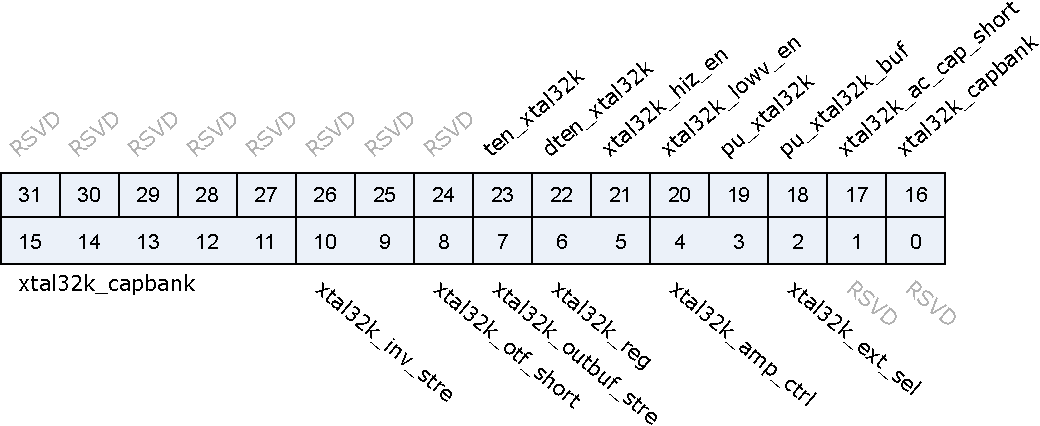
\includegraphics{HBN_xtal32k.pdf}
\end{figure}

\regdes{31:24&RSVD& & & \\\hline
23&ten\_xtal32k&r/w&1'h0&\\\hline
22&dten\_xtal32k&r/w&1'h0&\\\hline
21&xtal32k\_hiz\_en&r/w&1&high-z xtal32k input/output for share gpio usage\\\hline
20&xtal32k\_lowv\_en&r/w&1'h0&xtal32k low voltage mode enable\\\hline
19&pu\_xtal32k&r/w&0&power up signal for 32K crystal oscillator\\\hline
18&pu\_xtal32k\_buf&r/w&1&1: power up XTAL32k level shifter buffer\\\hline
17&xtal32k\_ac\_cap\_short&r/w&0&\\\hline
16:11&xtal32k\_capbank&r/w&6'h20&32K crystal load cap control word (also copy from efuse)\\\hline
10:9&xtal32k\_inv\_stre&r/w&2'h1&32K crystal inverter amplify strength\\\hline
8&xtal32k\_otf\_short&r/w&0&32K crystal over tone filter short\\\hline
7&xtal32k\_outbuf\_stre&r/w&0&32K crystal output buffer strength\\\hline
6:5&xtal32k\_reg&r/w&2'h1&32K crystal voltage regulator level\\\hline
4:3&xtal32k\_amp\_ctrl&r/w&2'h1&32K crystal oscillation amplitude control\\\hline
2&xtal32k\_ext\_sel&r/w&0&External 32K clock enable\\\hline
1:0&RSVD& & & \\\hline

}
